\subsection{Prueba de aceptación}
Esta prueba está basada en modelo de pruebas \textit{Game Flow}\cite{gameflow}. 
\textit{Game Flow} utiliza estrategias heurísticas de usabilidad y experiencia de usuario.
Este modelo permite medir varios aspectos de los cuales en este proyecto se probarán: 
 {\it joyment} (disfrute), diseño de interfaces, mecánicas y jugabilidad. 
 
Se tomo la decisión de aplicar las pruebas \textit{Game Flow} por nivel ....
 
Esta prueba de aceptación se dividió en dos partes: .... presencial y en línea.


 
\subsubsection{Objetivo} %% debe concordar con la parte de arriba.
Obtener la opinión de los usuarios sobre los elementos de un nivel, tales como
la mecánica, la jugabilidad, las interfaces, los enemigos, etc.

\subsubsection{Herramientas}

Para aplicar las pruebas se utilizaron .... %describir las herramientas
Apk del juego, cuestionario(ver anexo \ref{Anexo:Cuestionario}) y encuesta en \textit{Google Docs}.

\subsubsection{Aplicación}
Para estas pruebas se requieren grupos de personas para probar los niveles del
juego.

%Instrucciones <- crear subsubsection
Para realizar
la prueba se le proporciona al jugador el {\it link} para descargar la apk del juego
y el link de la encuesta. 

La prueba de aceptación está diseñada para ser la más larga, ya que
se busca que el mayor número de personas puedan probar el juego. %% replantearlo

Esta prueba se realiza de dos maneras diferentes:
\begin{itemize}
        \item Publicando los links de la apk y de la encuesta en redes sociales,
        indicando las instrucciones de responder la encuesta por nivel terminado.
        \item Realizando pruebas presenciales a grupos de personas.
\end{itemize}

En el caso de las pruebas presenciales, además de la encuesta se puede observar
las reacciones reales de lo jugadores mientras prueban el juego.

%% separar la aplicación de la conclusión. 
En muchos casos se pudo observar a diferentes grupos de amigos compitiendo por acabar el
nivel, jugadores gritando de alegría al acabar un nivel que les había costado
mucho esfuerzo o exclamaciones llenas de emoción al ser derrotados de último
momento por un jefe (ver figura \ref{fig:AlumnosESCOM}).
\begin{figure}
  \centering
 
   \subfigure[Dos alumnos de la Escuela Superior de Cómputo probando el juego.] {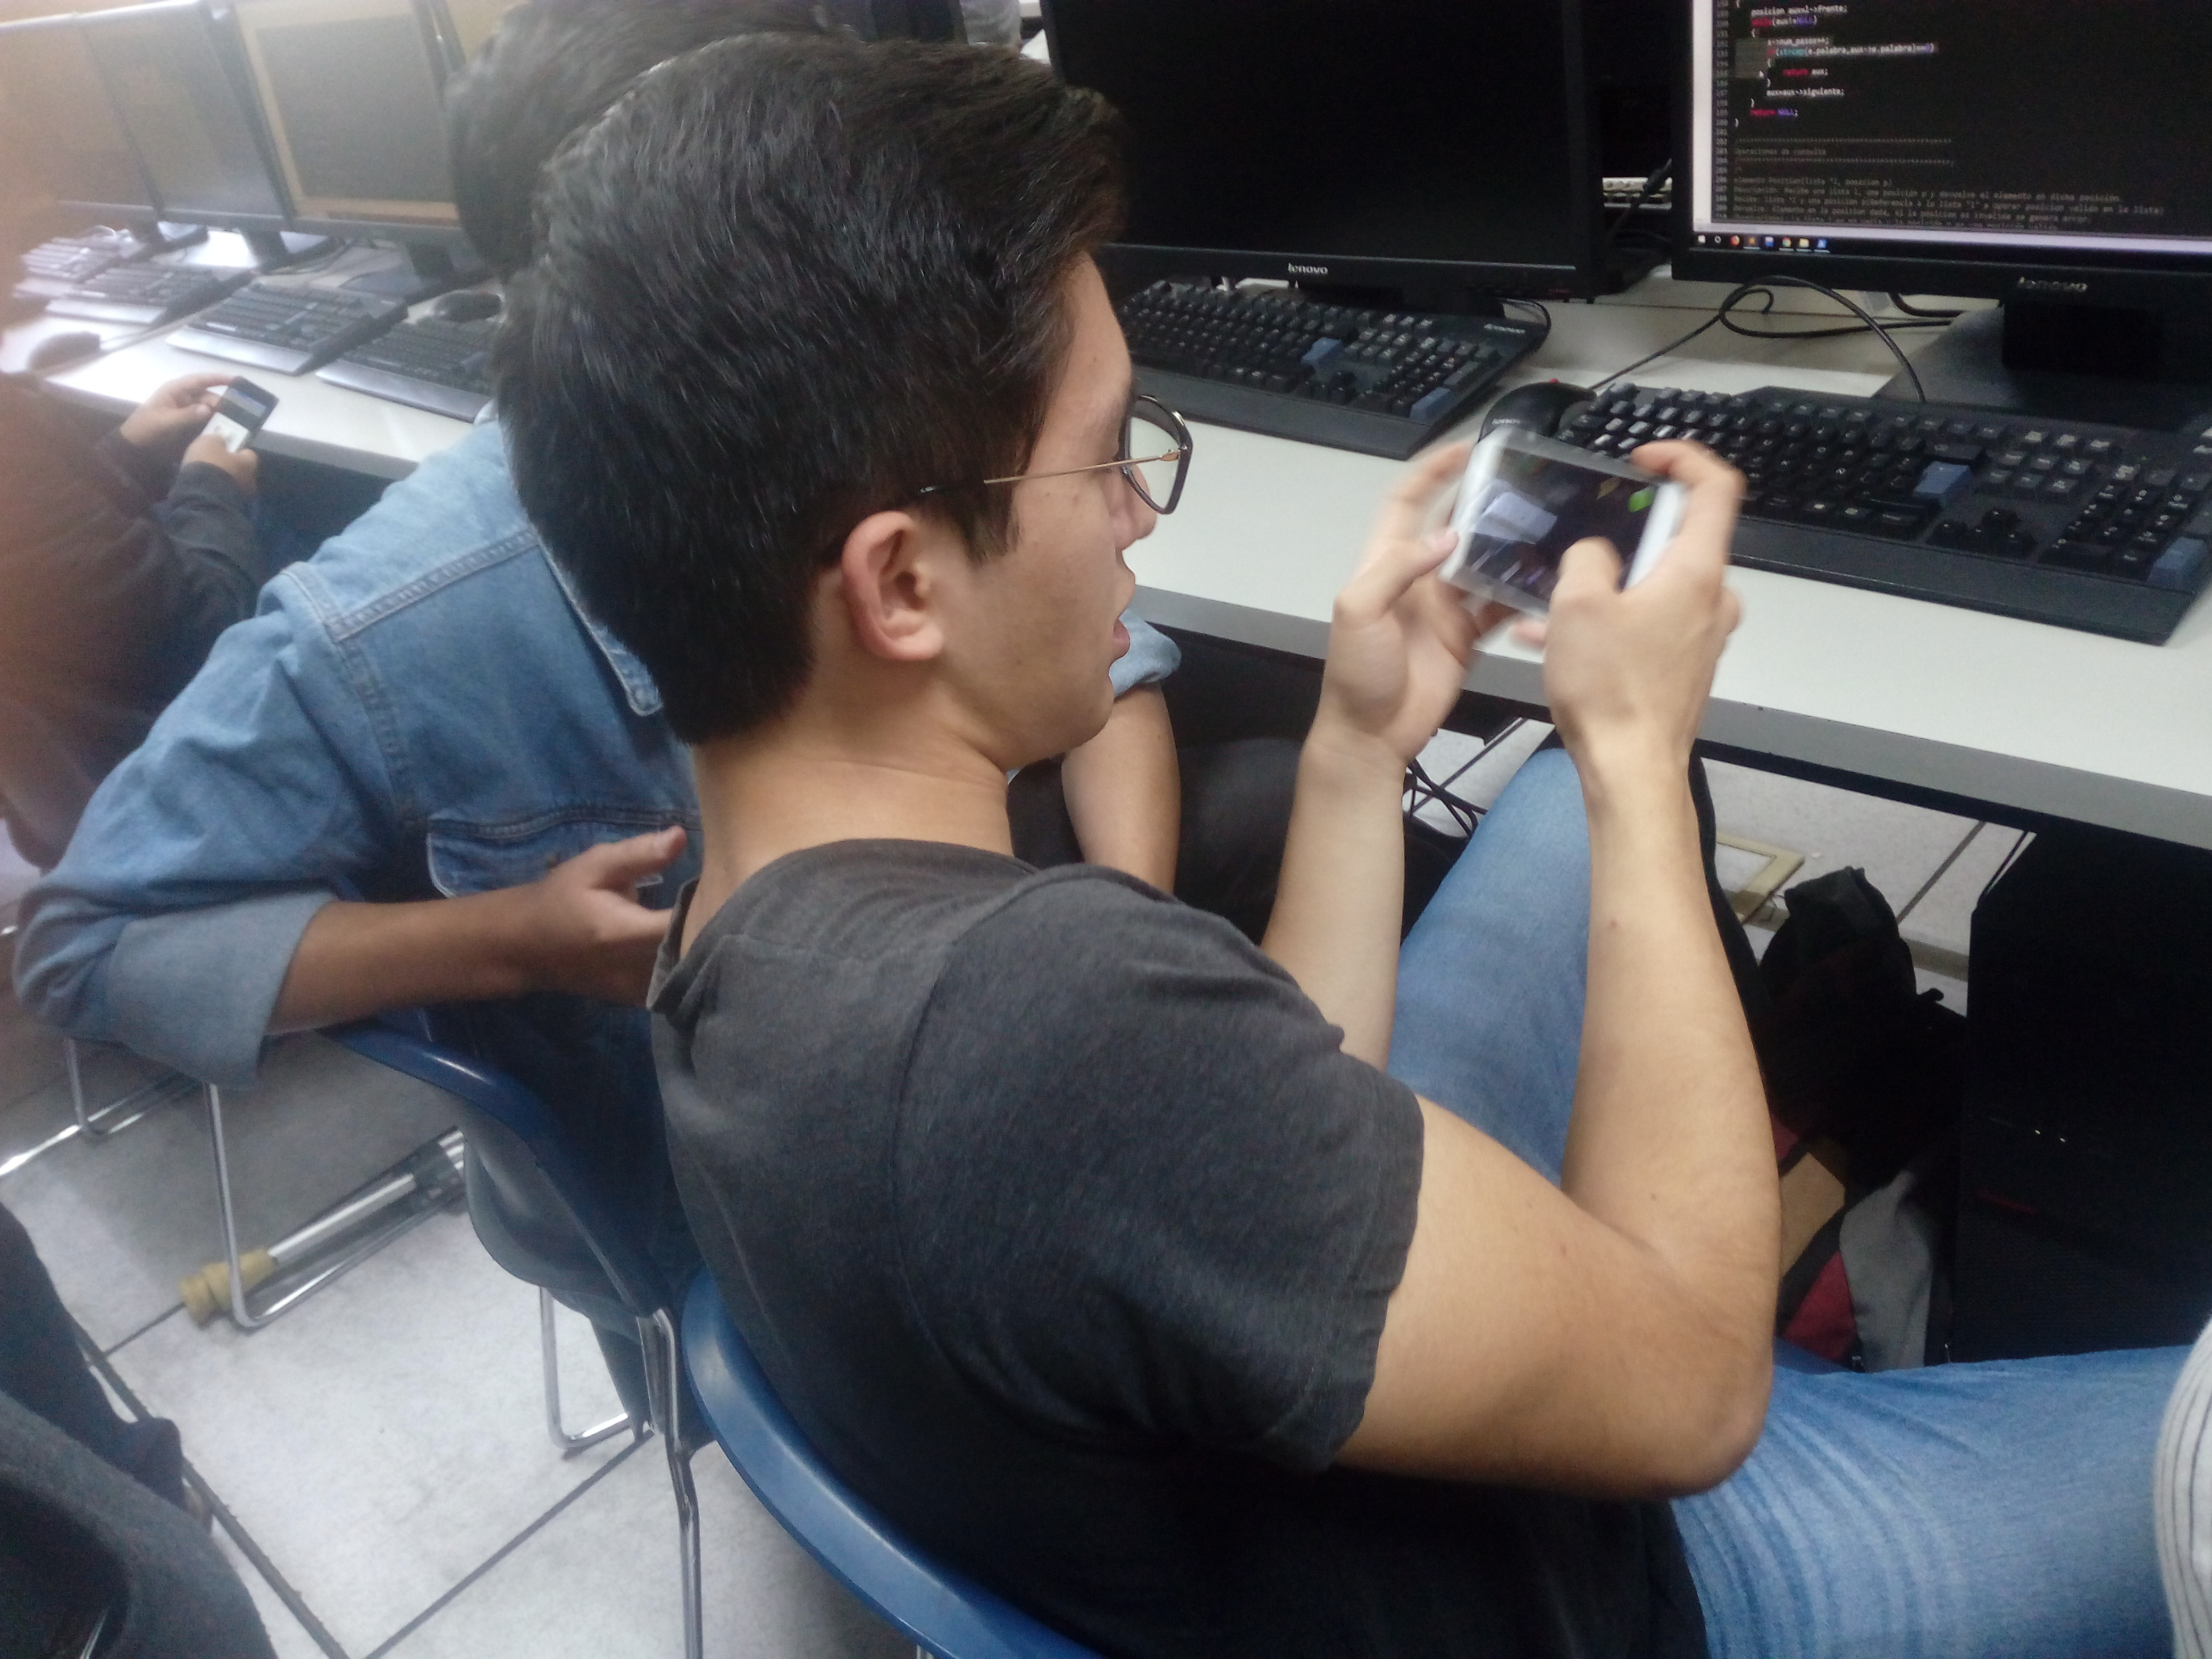
\includegraphics[width=0.4 \textwidth]
   {04ResultadosObetnidos/imagenes/usuarios01}}
        
        \subfigure[Grupo de alumnos de la Escuela Superior de Cómputo probando el
        juego.] {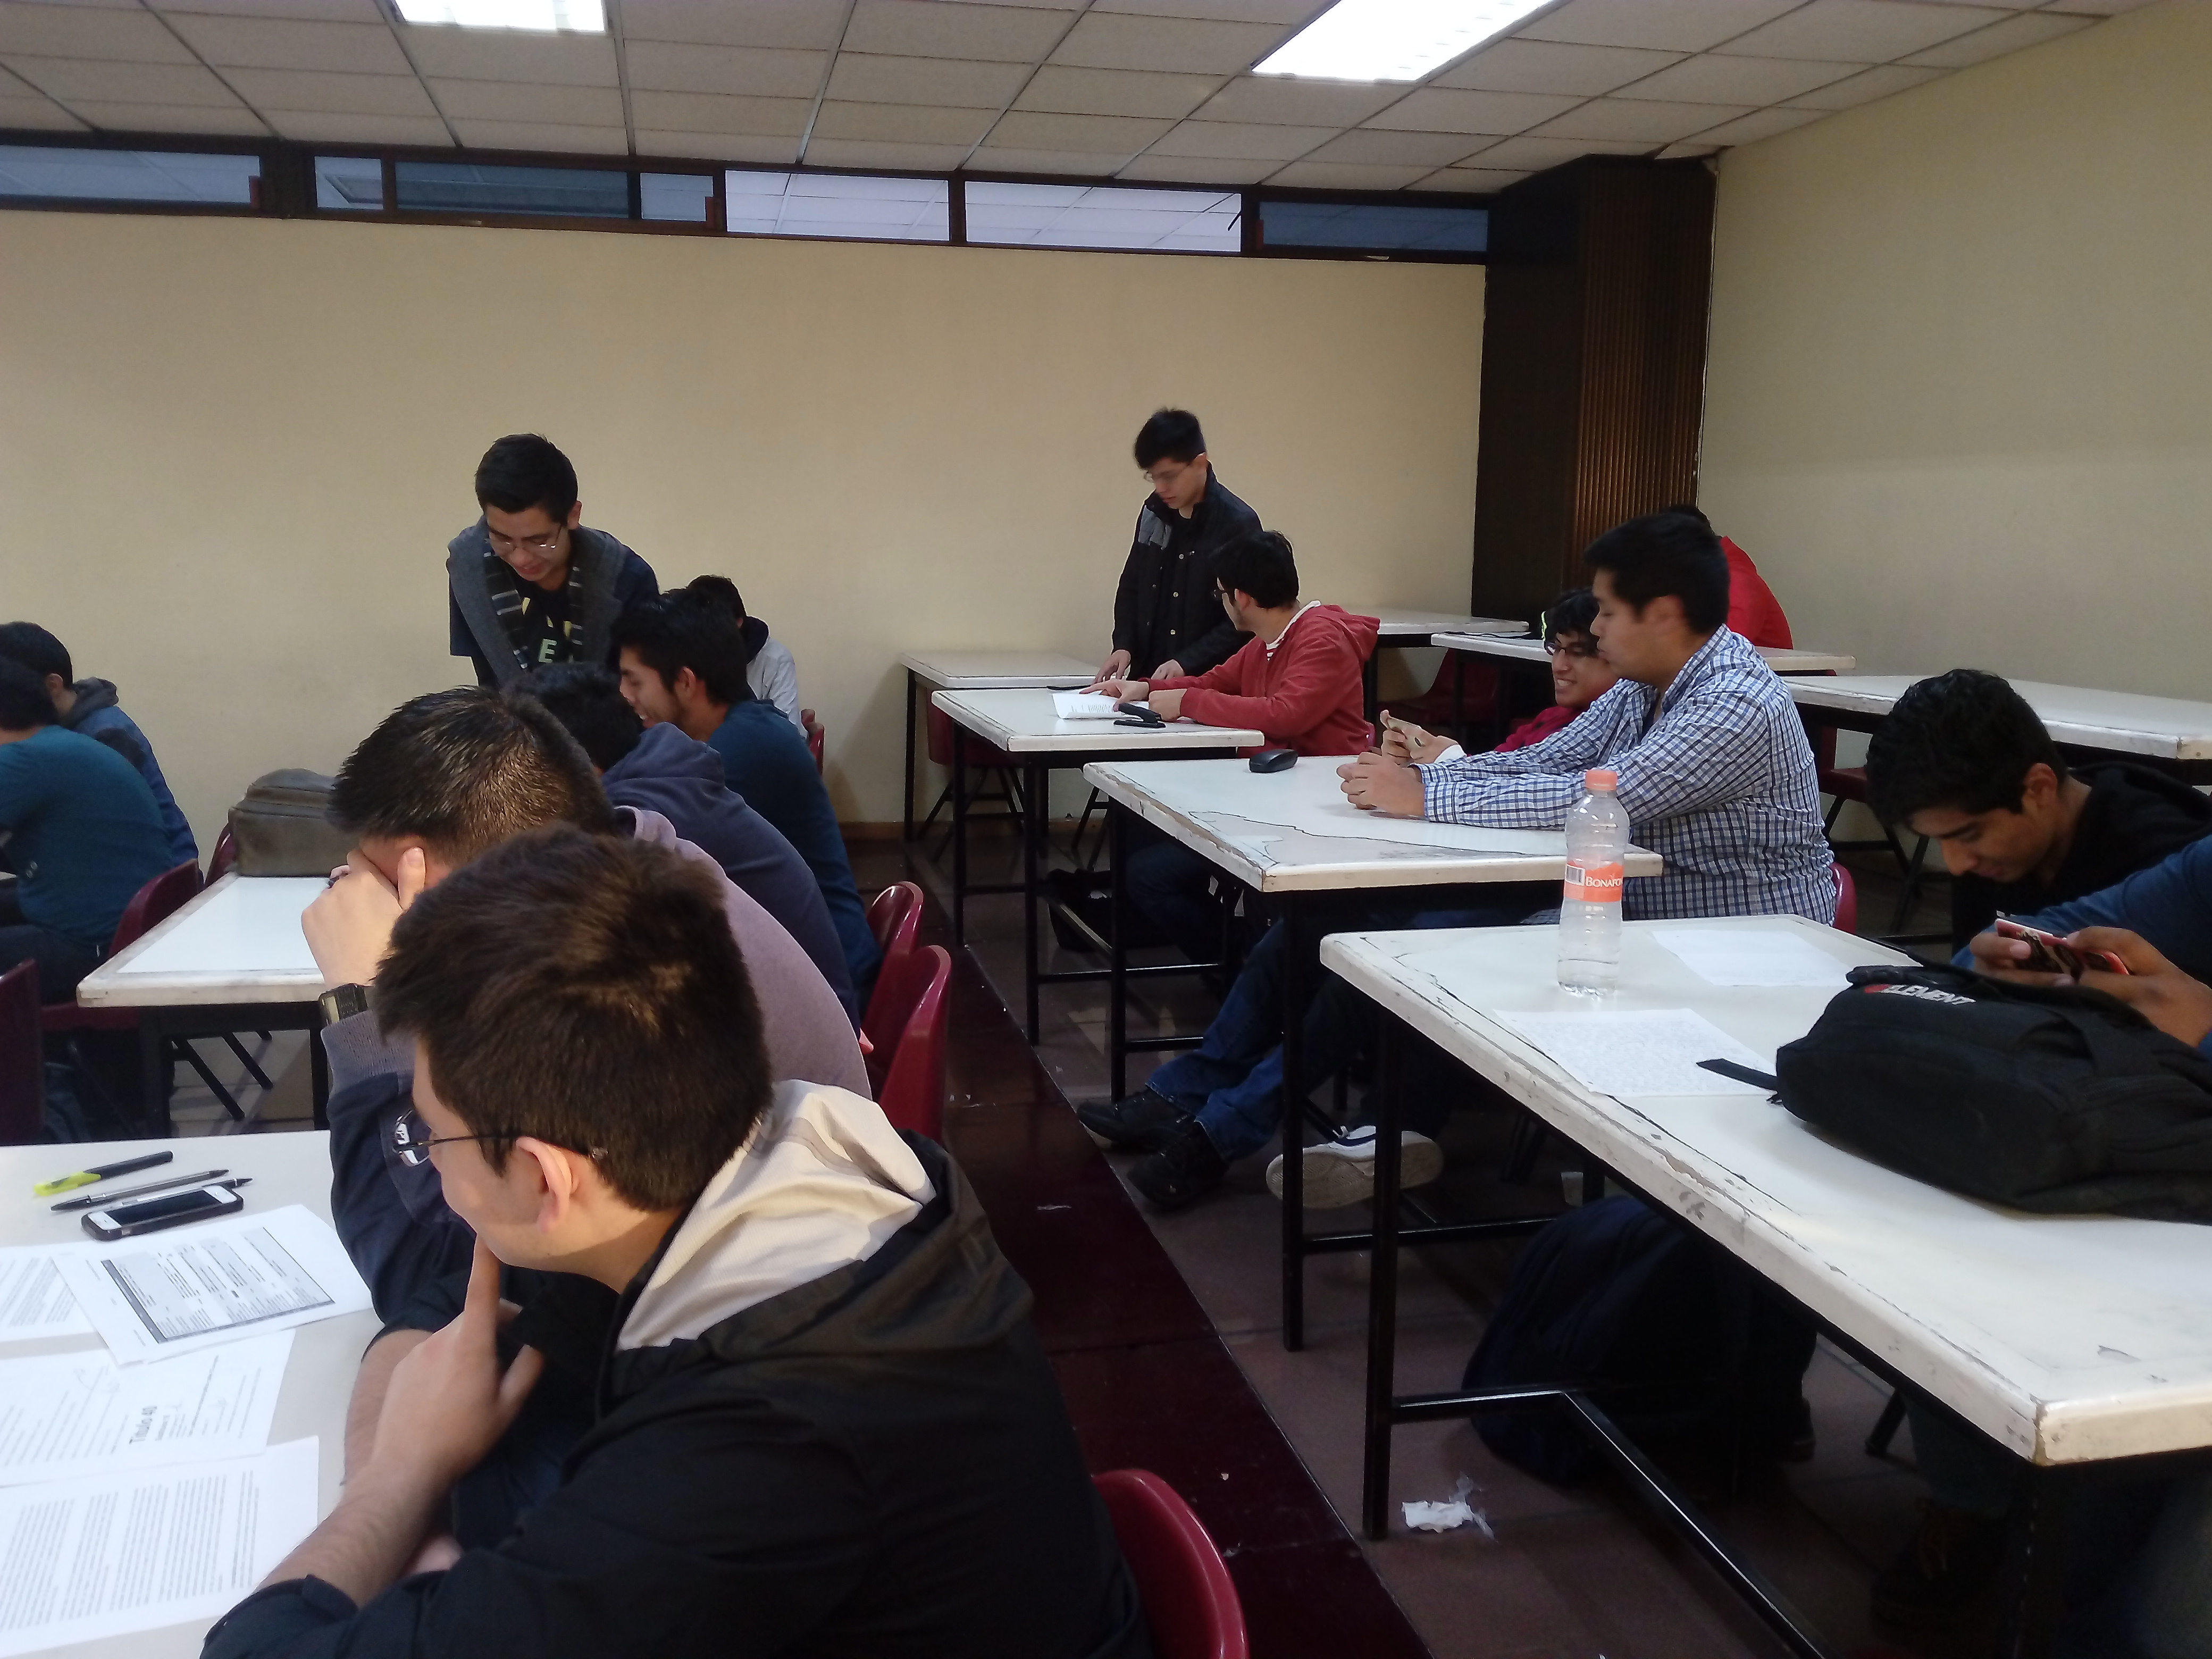
\includegraphics[width=0.4 \textwidth]{04ResultadosObetnidos/imagenes/usuarios02}}
  \caption{Resultados de la herramienta \textit{profiler} al analizar una cinemática.}
  \label{fig:AlumnosESCOM}
\end{figure}
\subsubsection{Conclusiones de la prueba}

A continuación se presentan algunos de los resultados de la encuesta, 
lo resultados completos se encuentran en ..... 
\begin{itemize} %% separar resultados de conclusiones
        \item La principal marca de dispositivos con el que fue probado el juego fue
        Motorola con sistema operativo Android 7.
        \item La mayoría de los usuarios consideran como bueno el movimiento del
        personaje, pero consideran que haciendo más estable el salto el control del
        personaje mejoraría.
        \item La mayoría de los usuarios consideran que la respuesta de la
        \textit{GUI} es buena; sin embargo, recomiendan mejorar el tiempo de respuesta
        de ésta y agregar una animación que indique que un botón ha sido oprimido.
        \item La mayoría de los usuarios opina que la actualización de la barra de
        tonali es buena pero les gustaría que existiera un indicador numérico para ver
        la cantidad de disparos que les queda.
        \item La mayoría de los usuarios considera que lo hace hace débil a un personaje
        es su patrón de movimiento y no la cantidad de daño que pueda generar; por
        otro lado también la mayoría de los usuarios considera que lo que hace a un
        enemigo fuerte es su patrón de movimiento.
        \item El Fantasma morado es considerado por muchos usuarios como el enemigo más
        poderoso en los niveles de plataforma, porque se si se deseara hacer niveles
        más difíciles este debería de ser el enemigo predominante.
        \item El fantasma rojo es considerado por muchos usuarios como el enemigo más
        débil en los niveles de plataforma, porque se si se deseara hacer niveles
        más fáciles este debería de ser el enemigo predominante.
        \item Las dos principales causas de muerte en los jugadores son el tiempo
        de respuesta de la \textit{GUI} y que los enemigos eran demasiado fuertes.
        \item La mayoría de los usuarios consideran sus muertes como un factor de reto
        en el juego. Considerando que la principal causa de muerte fue el tiempo de
        respuesta de la \textit{GUI}, se puede concluir que mejorando este factor se
        disminuiría el porcentaje de jugadores que consideran como factor de estrés su
        muerte.
\end{itemize}

Las conclusiones que se obtuvieron de las pruebas son:

%% sección aparte
Adicionalmente lo jugadores hicieron observaciones y peticiones que ellos
consideran podrían mejorar la experiencia de juego:
\begin{itemize}
        \item Animación que indique que un enemigo ha recibido daño.
        \item Barra de vida para los enemigos.
        \item Posibilidad de que el jugador se agache.
        \item Mensajes de confirmación para los botones que llevan al menú de selección 
        y que cierran la aplicación.
        \item Mejorar el comportamiento de los disparos.
\end{itemize}
Si se desean consultar las gráficas se puede consultar el anexo \ref{Anexo:resultados}.
